
%----------------------------------------------------------------
\begin{question}
    Considere la función

     \[
        f(x,y) =
        \begin{dcases}
            \frac{e^{x^{2}+y^{2}}-1}{\sqrt{x^{2}+y^{2}}} & \textnormal{si}\ (x,y) \neq (0,0) \\
            0                         & \textnormal{si}\ (x,y) = (0,0)
        \end{dcases}
    \]

    \begin{enumerate}
        \item Analizar la continuidad de $f$ en el origen
        \item Analizar la diferenciabilidad de $f$ en el origen.
        \item Analizar la existencia de las derivadas direccionales de $f$ en el origen.\\
    \end{enumerate}
\end{question}

%---------------------------------------------------------------------
\begin{question}
    Sean $f:\Rn{2}\to\R$ diferenciable, $g(x,y)=(xy^2,x^2-2y)$ y $h=f\circ g$. Sabiendo que $h(1,-1) = 2$ y que $\grad h(1,-1)=(2,-4)$, halle el plano tangente al gráfico de $f$ en el punto $(1,3,f(1,3))$.
\end{question}
%------------------------------------------------
\begin{question}
    Sean $f$ y $g$ dos campos escalares de clase $C^2$ tales que $f(1,2)=g(x,y)$, $\grad f(1,-1)=\grad g(2,-4)$ y $H_f(1,2)=H_g(1,2)$, calcular 
    
\[
        \lim_{(x,y)\to(1,2)} \
        \frac{f^2(x,y)-g^2(x,y)}{x^2+y^2-2x-4y+5}
    \]
\end{question}
%------------------------------------------------------------------
\begin{question}
    Hallar analíticamente los puntos más lejanos y más cercanos al origen del elipsoide dado por la ecuación {\large$\frac{x^2}{64}+\frac{y^2}{36}+\frac{z^2}{25}-1=0$}
\end{question}
%---------------------------------------------------------------------
\newpage

\begin{solution}
    En primer lugar analizamos la continuidad, como $f$ es una función partida, queremos demostrar que $f$ es continua en (0,0) si:  $\lim_{(x,y)\to(0,0)} \ f(x,y) = f(0,0)=0$

 
Utilizando el límite notable conocido:  $ \lim_{t\to 0} \
        (\frac{e^{t}-1}{t})=1$ , sabemos que 
\[
        \lim_{t\to 0} \
        \frac{e^{t}-1}{\sqrt{t}}=0 
    \]
    Pues, multiplicando arriba y abajo por $\sqrt{t}$, sabiendo que $t\neq 0$, tenemos que
    \[
        \lim_{t\to 0} \
        (\frac{e^{t}-1}{\sqrt{t}})(\frac{\sqrt{t}}{\sqrt{t}}) =\lim_{t\to 0} \
        (\frac{e^{t}-1}{t})\sqrt{t}=0
    \]
    Llamamos  $t(x,y)=x^{2}+y^{2}$ y sabemos que 
   \[
        \lim_{(x,y)\to(0,0)} t(x,y)=0
    \]
    Definimos $g(z)=\frac{e^{z}-1}{\sqrt{z}}=0 $ y realizando la composición $f(x,y)=g\circ t(x,y) \hspace{0.25cm}\forall (x,y)\in \mathbb{R}^ 2 -(0,0)$ tenemos que
\[
        \lim_{(x,y)\to (0,0)} \
        g\circ t(x,y)=\lim_{(x,y)\to (0,0)} \
        g(t(x,y))=\lim_{t\to 0} \
        \frac{e^{t}-1}{\sqrt{t}}=0 
    \]
    
   $\therefore f$ es continua en $(0,0)$
   

    Para analizar la diferenciabilidad de $f$ en el (0,0) en primer lugar vamos a evaluar la existencia de las derivadas direccionales, siendo $\vec{u}=(u_1,u_2)$ con $|\vec{u}|=1$
    
  \[
\displaystyle\frac{\partial f}{\partial \vec{u}}(0,0)=  \lim_{h\to 0} \
        \frac{f((0,0)+h\vec{u})-f(0,0)}{h}=  \lim_{h\to 0} \
        \frac{f(hu_1,hu_2)-f(0,0)}{h}= \lim_{h\to 0} \
        \frac{e^{h^2u_1^2+h^2u_2^2}-1}{h\sqrt{h^2u_1^2+h^2u_2^2}} 
 \]
 
  Sabemos que 
         \[
       |\vec{u}|=1   \iff \sqrt{u_1^2+u_2^2}=1  \iff u_1^2+u_2^2 =1
        \]
         
          Por lo cuál
 \[
\displaystyle\frac{\partial f}{\partial \vec{u}}(0,0)=   \lim_{h\to 0} \
        \frac{e^{h^2}-1}{h|h|} = \lim_{h\to 0} \
        \frac{e^{h^2}-1}{h^2}\frac{h}{|h|}
 \]

Tomando límites laterales
\[
\lim_{h\to 0^+} \
        \frac{e^{h^2}-1}{h^2}\frac{h}{|h|}=1
        \]
\[   
    \lim_{h\to 0^-} \
    \frac{e^{h^2}-1}{h^2}\frac{h}{|h|}=-1 
\]
 Como los límites laterales son distintos, entonces podemos afirmar que $\nexists   $ 
  $ \displaystyle\frac{\partial f}{\partial \vec{u}}(0,0)    $       $     \forall \vec{u} /|\vec{u}|=1$ , al no existir las derivadas direccionales de $f$ en $(0,0)$, las parciales tampoco.

  $\therefore $  $f$ no es diferenciable en $(0,0)$
\end{solution}
\newpage
\begin{solution}

    Como   $f:\Rn{2}\to\R$ es diferenciable en todo su dominio por ser composición de funciones diferenciables,  la ecuaci\'on de su plano tangente en el punto $(1,3)$ est\'a dada por
    \begin{equation}
        z= f(1,3) + \grad f(1,3) (x-1,y-3),  \label{eq:zNabla}
    \end{equation}   luego ser\'a  suficente con encontar $ f(1,3)$ y $\grad f(1,3).$

    Por un lado,      $h(1,-1)= f\circ g (1,-1) =  f(1,3)=2$  y por otro lado,  como $f$ y $g$ son ambas diferenciables,  por la regla de la cadena,  tenemos que
    \begin{equation}
        \grad h(1,-1)=\grad (f\circ g)(1,-1)=\grad f(g(1,-1)) \:\boldsymbol{D}_g(1,-1) = \grad f (1,3) \:\boldsymbol{D}_g(1,-1),  \label{eq:hNabla}
    \end{equation}    donde $\boldsymbol{D}_g$ es la matriz diferencial o  jacobiana de $g$.

    \noindent  Hallemos $\boldsymbol{D}_g$
    \begin{align*}
        \boldsymbol{D}_g(1,-1) & =
        \left(\begin{array}{cc}
                      \displaystyle\partialx (xy^2)            & \displaystyle\partialy (xy^2)           \\[10pt]
                      \displaystyle\partialx  (x^2 -2y) & \displaystyle\partialy (x^2 -2y)
                  \end{array}\right)\left.\rule{0pt}{1.1cm}\right\rvert_{(1,-1)}             \\[2pt]
                              & =\left(\begin{array}{cc}
                                               \displaystyle y^2                 & \displaystyle 2xy              \\[5pt]
                                               \displaystyle   2x & \displaystyle -2
                                           \end{array}\right)\left.\rule{0pt}{0.7cm}\right\rvert_{(1,-1)} \\[2pt]
                              & =\left(\begin{array}{cc}
                                               1    & -2    \\
                                               2 & -2
                                           \end{array}\right)
    \end{align*}
    Luego, reemplazando en  a   \eqref{eq:hNabla}
    \[
        \grad h(1,-1) = \grad f(1,3)\left(\begin{array}{cc}
                1   & -2    \\
                2 & -2
            \end{array}\right) = \left(f_x(1,3) + 2f_y(1,3),\;-2f_x(1,3)-2f_y(1,3)\right)
    \]

    y con la información de la consigna, se despejan
    \[\begin{cases}
            \;f_x(1,3) + 2f_y(1,3)=2 \\[5pt]
            \;-2f_x(1,3)- 2f_y(1,3)=-4
        \end{cases}
        \iff
        \begin{cases}
            \;f_x(1,3)=2 \\[5pt]
            \;f_y(1,3)=0
        \end{cases}
    \]
    $\therefore\quad\grad f(1,3)=(2,0)$.

       Reemplazando en \eqref{eq:zNabla}
      \[
        z= 2 + (2,0)(x-1,y-3)
    \]


        Despejando, la ecuación del plano tangente al grafico de $f$ en el punto $(1,3,f(1,3))$ es
          \[
         z -2x = 0
    \]
 
\newpage
\end{solution}

\begin{solution}
   En primer lugar, reescribimos el límite pedido 
   \[
        \lim_{(x,y)\to(1,2)} \
        \frac{(f-g)_{(x,y)}(f+g)_{(x,y) }}{|(x-1,y-2)|^2}
    \]
    Dado que $f$  y $g$ son dos campos escalares de clase  $C^2(\mathbb{R}^2)$,  se define  el polinomio de Taylor de primer orden centrado en $(1,2)$ de ambas funciones, que noteremos por $P_2[f,(1,2)]$ , $P_2[g,(1,2)]$ como,
    \begin{equation}
        P_2[f,(1,2)](x,y)=f(1,2)+\grad f(1,2)\cdot(x-1,y-2)+ \frac{1}{2}(x,y)\boldsymbol{H}_f(c_1,c_2)\begin{pmatrix}x-1\\y-2\end{pmatrix}, \label{eq:polTay2}
    \end{equation}
    \begin{equation}
        P_2[g,(1,2)](x,y)=f(1,2)+\grad f(1,2)\cdot(x-1,y-2)+ \frac{1}{2}(x,y)\boldsymbol{H}_f(c_1',c_2')\begin{pmatrix}x-1\\y-2\end{pmatrix}, \label{eq:polTay2}
    \end{equation}
Sabemos que
\[
        (f-g)_{(x,y)}=  P_2[(f-g),(1,2)](x,y) + R_2[(f-g),(C,(x-1,y-2)] 
    \]
  

Utilizando los datos de enunciado, podemos ver que
\[
       P_2[(f-g),(1,2)](x,y)= (f-g)_{(1,2)}+\grad (f-g)_{(1,2)}\cdot(x-1,y-2)+ \frac{1}{2}(x-1, y-2)^t\boldsymbol{H}_(f-g)_{(C)}\begin{pmatrix}x-1\\y-2\end{pmatrix} =0
    \]
    \[
      \Rightarrow 
        (f-g)_{(x,y)}=  R_2[(f-g),(C,(x-1,y-2)] 
    \]

    Ademas, sabemos que,
  
    \[
        \lim_{(x,y)\to(1,2)} \
        \frac{R_2[(f-g),(C,(x-1,y-2)]}{|(x-1,y-2)|^2}=0
    \]

Utilizando los datos recien mencionados, y sabiendo que $ \lim_{(x,y)\to(1,2)} \
        (f+g)_{(x,y) }=L \in \mathbb{R} $ calculamos el limite solicitado

  \[
        \lim_{(x,y)\to(1,2)} \
        \frac{(f-g)_{(x,y)}(f+g)_{(x,y) }}{|(x-1,y-2)|^2}=\lim_{(x,y)\to(1,2)} \
        \frac{R_2[(f-g),(C,(x-1,y-2)]. (f+g)_{(x,y) }}{|(x-1,y-2)|^2}=0
    \]
    
    
 
\end{solution}

\begin{solution}
    En este ejercicio debemos hallar los puntos mas lejanos y mas cercanos al origen de la funcion que denominaremos $g(x,y,z)=\frac{x^2}{64}+\frac{y^2}{36}+\frac{z^2}{25}-1$ , para lo cual utilizaremos la funcion distancia: $f(x,y)=\sqrt{x^2+y^2+z^2}$ \newline Busco los minimos de $f$ restringidos al conjunto de nivel $g(x,y,z)=0$ utilizando los multiplicadores de lagrange
\[
        \grad f(x,y)=\lambda \grad g(x,y,z)
    \]
    \[
        (2x,2y,2z)=\lambda (\frac{2x}{64},\frac{2y}{36},\frac{2z}{25}) \iff \begin{cases}
            x = \lambda\frac{x}{64}\\
            y = \lambda\frac{y}{36}\\
            z = \lambda\frac{z}{25}
        \end{cases}
    \]
    
    Estas ecuaciones implican que 2 variables deben ser nulas para que el sistema tenga solucion, entonces:

1- Si $x\neq 0 \land y=0 \land z=0 \Rightarrow \lambda=64  \Rightarrow x=\pm 8$ 

2- Si $y\neq 0 \land x=0 \land z=0 \Rightarrow \lambda=36  \Rightarrow y=\pm 6$ 

2- Si $z\neq 0 \land x=0 \land y=0 \Rightarrow \lambda=36  \Rightarrow y=\pm 5$ 

    De esta manera, encontramos 6 posibles maximos y minimos de la funcion $f$
\[
        P_1=(8,0,0) 
         \]
         \[
        P_2=(-8,0,0) 
         \]
        \[
        P_3=(0,6,0) 
         \]
         \[
        P_4=(0,-6,0) 
         \]
         \[
        P_5=(0,0,5) 
         \]
         \[
        P_6=(0,0,-5) 
    \]
    
    Por el teorema de valores extremos de Weierstrass, sean $A \subset \mathbb{R}^3$ conjunto cerrado y acotado y $f:A\subset\mathbb{R}^3\rightarrow\mathbb{R} $ funcion continua, entonces f alcanza un maximo y minimo absoluto en $A$.
    
    De esta manera, reemplazando los puntos en $f$ encontramos los maximos y minimos de la misma, restringida en $A$ (conjunto de nivel 0 de $g)$. Entonces podemos ver que los puntos mas alejados del origen son el $(8,0,0)$ y el $(-8,0,0)$ , y que los mas cercanos son el $(0,0,5)$  y el $(0,0,-5)$ \newline
    
    Tambien, se puede ver de forma grafica
\begin{figure}[h!] % El entorno figure te permite incluir imágenes
    \centering
    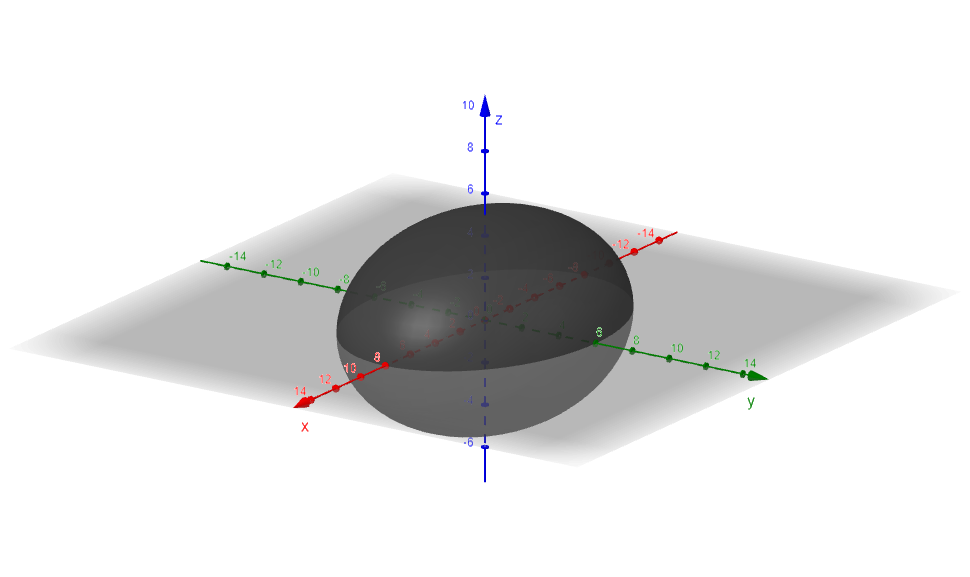
\includegraphics[width=0.75\textwidth]{../figs/Grafico_elipsoide.png}
    \caption{Grafica de $g(x,y,z)$.}
    \label{fig:ejemplo} % Etiqueta para hacer referencia a la imagen
\end{figure}

\end{solution}


